\documentclass[a4paper, 12pt, twoside, openright]{article}
\usepackage[T1]{polski}
\usepackage[utf8]{inputenc}
\newtheorem{theorem}{Twierdzenie}
\usepackage{helvet}
\usepackage{graphicx}
\usepackage{color}
\usepackage{subfig}
\usepackage[table, svgnames, dvipsnames]{xcolor} 
\usepackage{array}
\usepackage{float}
\usepackage{cellspace}
\usepackage[top=1.3in,bottom=1.3in,right=1in,left=1in,headheight=95pt,headsep=-0.5cm]{geometry}
\usepackage{color}
\usepackage{listings}
\usepackage{caption}
\usepackage{cmap}

\usepackage{enumitem}
\setlist{nolistsep}
\usepackage{hyperref}
\usepackage{listings}

\definecolor{mGreen}{rgb}{0.596,0.592,0.102}
\definecolor{mText}{rgb}{0.235,0.22,0.212}
\definecolor{mGray}{rgb}{0.5,0.5,0.5}
\definecolor{mPurple}{rgb}{0.58,0,0.82}
\definecolor{backgroundColour}{rgb}{0.984,0.945,0.78}

\lstdefinestyle{CStyle}{
    commentstyle=\color{mGreen},
    keywordstyle=\color{magenta},
    numberstyle=\tiny\color{mGray},
    stringstyle=\color{mPurple},
    basicstyle=\footnotesize\color{mText},
    breakatwhitespace=false,
    breaklines=true,
    captionpos=b,
    keepspaces=true,
    numbers=left,
    numbersep=5pt,
    showspaces=false,
    showstringspaces=false,
    showtabs=false,
    tabsize=2,
    language=C
}

\lstdefinestyle{CStyleLine}{
    commentstyle=\color{mGreen},
    keywordstyle=\color{magenta},
    numberstyle=\tiny\color{mGray},
    stringstyle=\color{mPurple},
    basicstyle=\footnotesize,
    breakatwhitespace=false,
    breaklines=true,
    captionpos=b,
    keepspaces=true,
    numbersep=5pt,
    showspaces=false,
    showstringspaces=false,
    showtabs=false,
    tabsize=2,
    language=C
}


\newcounter{nalg} 
\DeclareCaptionLabelFormat{algocaption}{Algorytm \thenalg}
\lstnewenvironment{algorithm}[1][] 
{   
	\refstepcounter{nalg}
	\captionsetup{labelformat=algocaption,labelsep=colon} 
	\lstset{ 
		mathescape=true,
		frame=tB,
		numbers=left, 
		numberstyle=\tiny,
		basicstyle=\scriptsize, 
		keywordstyle=\color{black}\bfseries\em,
		keywords={,input, def, output, return, datatype, function, in, if, else, foreach, while, begin, end }
		numbers=left,
		xleftmargin=.04\textwidth,
		#1 
	}
}
{}



\begin{document}

\lstset{language=Python}
% =====  STRONA TYTULOWA  ====

\thispagestyle{empty}
\vspace*{-0.6in}
%% ------------------------ NAGLOWEK STRONY =======================------

\includegraphics[height=37.5mm]{img/logo_agh}\\
\rule{30mm}{0pt}
{\large\textsf{Wydział Fizyki i Informatyki Stosowanej}}\\
\rule{\textwidth}{3pt}\\
\rule[2ex]
{\textwidth}{1pt}\\
\vspace{3ex}
\begin{center}
{\bf\LARGE\textsf{Praca inżynierska}}\\
\vspace{13ex}
% ======================= IMIE I NAZWISKO =======================----
{\bf\Large\textsf{Patryk Chodur}}\\
\vspace{3ex}
{\sf \small kierunek studiów:} {\bf\small\textsf{informatyka stosowana}}\\
\vspace{15ex}
%% ------------------------ TYTUL PRACY --------------------------------------
{\bf\huge\textsf{Opracowanie wtyczki do dekodowania
	pakietów Ethernet z~wykorzystaniem oprogramowania Wireshark
}}\\
\vspace{14ex}
%% ------------------------ OPIEKUN PRACY ------------------------------------
{\sf \Large Opiekun:} {\bf\Large\textsf{dr hab. inż. Bartosz Mindur}}\\
\vspace{22ex}
\textsf{\bf\large\textsf{Kraków, styczeń 2021}}
\end{center}


\newpage

%% =====  Oświadczenie =========
\begin{center}
	{\bf\large\textsf{Oświadczenie studenta}}
\end{center}


{\sf Uprzedzony(-a) o odpowiedzialności karnej na podstawie art. 115 ust. 1 i 2 ustawy z dnia 4 lutego 1994 r. o prawie autorskim i prawach pokrewnych (t.j. Dz. U. z 2018 r. poz. 1191 z późn. zm.): „Kto przywłaszcza sobie autorstwo albo wprowadza w błąd co do autorstwa całości lub części cudzego utworu albo artystycznego wykonania, podlega grzywnie, karze  ograniczenia wolności albo pozbawienia wolności do lat 3. Tej samej karze podlega, kto rozpowszechnia bez podania nazwiska lub pseudonimu twórcy cudzy utwór w wersji oryginalnej albo w postaci opracowania, artystyczne wykonanie albo publicznie zniekształca taki utwór, artystyczne wykonanie, fonogram, wideogram lub nadanie.”, a także uprzedzony(-a) o odpowiedzialności dyscyplinarnej na podstawie art. 307 ust. 1 ustawy z dnia 20 lipca 2018 r. Prawo o szkolnictwie wyższym i nauce (Dz. U. z 2018 r. poz. 1668 z późn. zm.) „Student podlega odpowiedzialności dyscyplinarnej za naruszenie przepisów obowiązujących w uczelni oraz za czyn uchybiający godności studenta.”, oświadczam, że niniejszą pracę dyplomową wykonałem(-am) osobiście i samodzielnie i nie korzystałem(-am) ze źródeł innych niż wymienione w pracy

\bigskip

Jednocześnie Uczelnia informuje, że zgodnie z art. 15a ww. ustawy o prawie autorskim i prawach pokrewnych Uczelni przysługuje pierwszeństwo w opublikowaniu pracy dyplomowej studenta. Jeżeli Uczelnia nie opublikowała pracy dyplomowej w terminie 6 miesięcy od dnia jej obrony, autor może ją opublikować, chyba że praca jest częścią utworu zbiorowego. Ponadto Uczelnia jako podmiot, o którym mowa w art. 7 ust. 1 pkt 1 ustawy z dnia 20 lipca 2018 r. — Prawo o szkolnictwie wyższym i nauce (Dz. U. z 2018 r. poz. 1668 z późn. zm.), może korzystać bez wynagrodzenia i bez konieczności uzyskania zgody autora z utworu stworzonego przez studenta w wyniku wykonywania obowiązków związanych z odbywaniem studiów, udostępniać utwór ministrowi właściwemu do spraw szkolnictwa wyższego i nauki oraz korzystać z utworów znajdujących się w prowadzonych przez niego bazach danych, w celu sprawdzania z wykorzystaniem systemu antyplagiatowego. Minister właściwy do spraw szkolnictwa wyższego i nauki może korzystać z prac dyplomowych znajdujących się w prowadzonych przez niego bazach danych w zakresie niezbędnym do zapewnienia prawidłowego utrzymania i rozwoju tych baz oraz współpracujących z nimi systemów informatycznych.}

\vspace{14ex}

\begin{center}

~~~~~~~~~~~~~~~~~~~~~~~~~~~~~~~~~~~~~~~~~~~~~~~~~~~~~~~~~~~~~~~~~ 
................................................................. \\
~~~~~~~~~~~~~~~~~~~~~~~~~~~~~~~~~~~~~~~~~~~~~~~~~~~~~~~~~~~~~~~  {\sf (czytelny podpis)} \\

\end{center}

%% =====  TYL STRONY TYTULOWEJ   ====


%% ============ OCENA OPIEKUNA =============
\newpage
\linespread{1.3}
\selectfont

\hspace*{\fill}\large{Ocena merytoryczna opiekuna}

\vspace{85mm}

%% ============ OCENA RECENZENTA =============
\newpage
\linespread{1.3}
\selectfont

\hspace*{\fill}\large{Ocena merytoryczna recenzenta}

\vspace{85mm}


%% ====== SPIS TRESCI ==========
\newpage
\tableofcontents


%=======================- 1 =======================
\newpage
\section{Wstęp}

TODO: napisać wstęp.


	\newpage
	\subsection{Cel pracy}

	\indent\par
	Celem pracy jest wykonanie dekodera pakietów bazujących na protokole UDP i~przenoszących konkretne dane pomiarowe.
	Dekoder powinien napisany być jako wtyczka do programu Wireshark napisana w języku C. Użycie tego języka umożliwia efektywne
	przetwarzanie danych, a zaimplementowanie projektu jako wtyczki zapewnia szybszą rekompilację wtyczki,
	niewymagającą przekomilowywania całego programu. Gotowa wtyczka może zostać użyta z dowolną instalacją programu Wireshark,
	pod warunkiem zachowania zgodności co do systemu operacyjnego i~wersji programu. Instalacja polega na przekopiowaniu
	pojedyńczego pliku do katalogu wtyczek programu. Alternatywą dla takiego rozwiązania jest stworzenie wbudowanego dekodera,
	ale ze względu na liczne wady - m.~in.: dłuższy czas rekompilacji oraz konieczność ingerencji w~kod źródłowy programu - rozwiązanie
	to nie zostało zastosowane.

	Dane do zdekodowania pochodzą z urządzenia GEMROC ASIC.

	TODO: coś o urządzeniu GEMROC ASIC.

	Każdy pakiet ma stałą długość -- 1500 bajtów całego pakietu, 1458 bajtów danych protokołu UDP.
	Dane przekazywane są protokołem UDP na porcie 48350.
	W dalszej części pracy autor odnosił się będzie do pakietu jako do sekcji danych pakietu UDP.

	Struktura danych pakietu określona jest następująco:
	\begin{itemize}
		\item 8 bajtów -- numer porządkowy pakietu. Jest on unikalny dla każdego pakietu i identyfikuje go w jednoznaczny sposób.
			Pakietom transmisji nadawane są kolejne liczby porządkowe.
		\item 8 bajtów -- pole status pakietu. Znajdują się w nim informacje na temat urządzenia GEMROC. Zawiera ono pola:
			\begin{itemize}
				\item Clk state
				\item I2C status
				\item ADC Clk sel
				\item ASIC enable status
			\end{itemize}
		\item 1440 bajtów -- sekcja danych pakietu. Jest ona wektorem 8 bajtowych pól danych. Pomimo stałej długości tej sekcji
			(jak i całego pakietu) ilość danych jest zmienna i określona w pakiecie. Maksymalna ilość danych możliwa do przeniesienia
			pojedyńczym pakietem wynosi 180. Każde pole danych składa się na:
			\begin{itemize}
				\item ADC
				\item Timestamp FPGA
				\item Timestamp ASIC
				\item Channel ID
				\item ASIC ID
				\item PileUp
				\item Overflow
			\end{itemize}
		\item 2 bajty -- ilość danych w sekcji danych. Trzy najmłodsze bity nie są używane, dlatego aby uzyskać właściwy wynik
			należy użyć przesunięcia bitowego w prawo o trzy bity.
	\end{itemize}


\newpage
\section{Opis zagadnienia}

	\subsection{Wprowadzenie}
	TODO: coś o internecie
	\subsection{Protokół UDP}
	TODO: coś o Udp
	\subsection{Sniffer -- analizator pakietów}
	\indent\par
	Sniffer, bądź analizator pakietów (ang. packet analyzer) to program komputerowy, którego celem jest przechwytywanie
	i monitorowanie ruchu internetowego. Umożliwia on
	podglądanie pakietów w celu ich analizy pod kątem zawartości, rozmiaru, zastosowania, bądź celu. Powodów do takiej
	analizy jest wiele. Użytkownik może chcieć badać komunikację dwóch urządzeń będących częścią autorskiego systemu
	informatycznego, sprawdzać zajętość łącza internetowego, debugować własną aplikację korzystającą z połączenia internetowego,
	lub podglądać ruch internetowy innego użytkownika.

	Na rynku dostępnych jest wiele przeznaczonych do tego celu narzędzi, różniących się funkcjonalnością, ceną czy licencją.
	Do najpopularniejszych z nich należą:
	\begin{itemize}
		\item \texttt{tcpdump} -- jeden z pierwszych snifferów, dostępny za darmo na 3-klauzulowej licencji BSD. Działa
			z większością systemów opartych na Unixie, bądź nim inspirowanych. Do obsługi używany jest wiersz poleceń.
			Pomimo nazwy wskazującej, ograniczoną możliwość pracy do protokołu TCP, działa także z pakietami UDP i innymi.
			Program rozwijany jest przez ,,The Tcpdump team'' i bazuje na wspólnie z nim rozwijanej bibliotece \texttt{libpcap}.
		\item \texttt{WinDump} -- port tcpdump na platformę Windows, udostępniony na tej samej licencji. Do przechywtywania
			pakietów używa biblioteki \texttt{WinPcap}, nawiązującej do \texttt{libpcap}.
		\item \texttt{ngrep} -- program będący przeniesieniem zasady działania komendy \texttt{grep} na ruch internetowy.
			Ze względu na użycie tej samej biblioteki do wyrażeń regularnych używa on składni \texttt{GNU grep}.
			Używa on własnej licencji podobnej do licencji BSD. Obsługuje popularniejsze protokoły takie jak TCP, UDP oraz IPv4.
		\item \texttt{Wireshark} -- darmowy i otwarty program do analizy ruchu internetowego. Wyposażony jest on w graficzny
			interfejs, dzięki czemu stanowi prostszą w obsłudze alternatywę dla \texttt{tcpdump}. Program bazuje na projekcie
			Ethereal, który nie jest już kontynuowany. Oparty jest on także na bibliotece
			\texttt{libpcap}. Program Wireshark wykorzystany jest zarówno
			do omówienia zagadnienia dekoderów w dalszej części wstępu, jak i w całej pracy. Udostępniony na licencji GPLv2.
	\end{itemize}

	\begin{minipage}{\linewidth}
		\begin{lstlisting}[style=CStyle,caption={Przykładowy output programu \texttt{tcpdump}}]
		tcpdump: data link type PKTAP
		tcpdump: verbose output suppressed, use -v or -vv for full protocol decode
		listening on pktap, link-type PKTAP (Apple DLT_PKTAP), capture size 262144 bytes
		18:19:53.799698 IP 17.248.147.206.https > 192.168.1.10.60104: Flags [.], ack 3811845539, win 330, options [nop,nop,TS val 810056002 ecr 1073857899], length 0
		18:19:53.799703 IP 17.248.147.206.https > 192.168.1.10.60104: Flags [.], ack 32, win 330, options [nop,nop,TS val 810056006 ecr 1073857944], length 0
		18:19:53.815484 IP m11373.contaboserver.net.27811 > 192.168.1.10.6881: UDP, length 97
		18:19:53.815988 IP 192.168.1.10.6881 > m11373.contaboserver.net.27811: UDP, length 312
		18:19:53.826779 IP 192.168.1.10.49212 > dns.google.domain: 21620+ PTR? 206.147.248.17.in-addr.arpa. (45)
		5 packets captured
		26 packets received by filter
		0 packets dropped by kernel \end{lstlisting}
	\end{minipage}


	Poza wspomnianymi dostępnych jest więcej narzędzi, w tym płatne, lecz popularność powyższych jest sprawia,
	że konieczność ich wspominania autor pracy uznał za nikłą.

	Jedną z podstawowych funkcjonalności snifferów jest podglądanie zawartości przechodzących przez łącze internetowe danych.
	W programie Wireshark dokonuje się jej za pomocą dekoderów (ang. dissector).

	\newpage
	\subsubsection{Dekodery}
	\indent\par
	Dekoder to część sniffera zajmująca się rozkodowywaniem pakietów określonego typu. Rozkodowywanie polega na intepretacji
	ciągu bajtów, jakim jest pakiet, i wyciąganiu z niego użytecznych informacji. Umiejscowienie danych, i ich znaczenie,
	charakterystyczne jest dla danego typu pakietu. Każdy typ pakietu wymaga więc dedykowanego dekodera, a aby rozkodowywać
	różne pakiety potrzebny jest ich zestaw.

	Pakiet może przenosić dane innego typu, które także wymagają rozkodowania. Przykładem może być pakiet TCP niosący pakiet
	http. Dekodery mają więc strukturę hierarchiczną -- wyjście jednego może stanowić wejście drugiego dekodera.

	\begin{figure}[h]
		\centering
			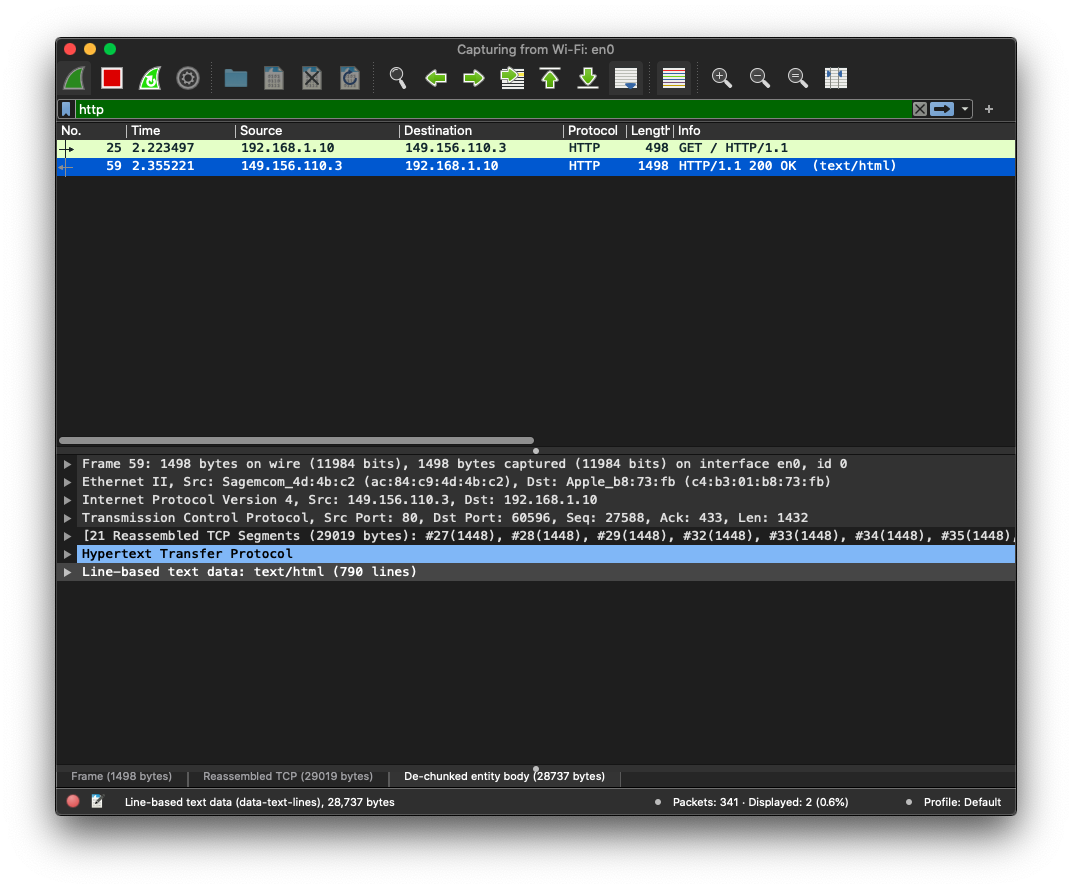
\includegraphics[width=1.0\textwidth]{img/screenshot_fis.png}
		\caption{Struktura pakietu http po otrzymaniu strony http://www.fis.agh.edu.pl}
		\label{fig:fis}
	\end{figure}

	Na rysunku (Rys.~\ref{fig:fis}) widać kolejne poziomy dekodowania pakietu http. Są to:

	\begin{itemize}
		\item Interfejs en0
		\item Protokół Ethernet
		\item Protokół IPv4
		\item Protokół TCP
		\item Dodatkowy poziom złożonych pakietów TCP
		\item Protokół http
		\item Dane tekstowe
	\end{itemize}

	Każdy dekoder jest osobnym modułem, dzięki czemu przykładowo dekoder http może także czytać dane idące protokołem UDP.
	Dekodery rejestrują zainteresowanie danymi pakietami dekoderowi wyżej w hierarchii, więc dekoder http może przykładowo
	żądać danych przesyłanych protokołem TCP na porcie 80. Istnieją także dekodery heurystyczne, cechujące się brakiem
	konieczności podawania konkretnych parametrów transmisji dekoderowi wyżej w hierarchii, oraz możliwością odrzucenia pakietu,
	aby mógł zostać użyty przez inny dekoder. Zostaną jednak one celowo, ze względu na znaczną złożoność i brak bezpośredniego
	związku z pracą, pominięte.

	Głównym zadaniem dekoderów, obok tworzenia hierarchii zawartości pakietu, jest wyświetlanie przesyłanych w pakiecie informacji w sposób zrozumiały dla użytkownika.
	Za pomocą interfejsu graficznego wyświetlają one zinterpretowane przez siebie dane transmisji. Sposób przedstawienia danych
	jest arbitralną decyzją programisty, podstawowymi więc kryteriami podczas ich projektowania powinny być użyteczność oraz czytelność.
	Programista może wzorować się na istniejących już rozwiązaniach, w szczególności dekoderach dołączonych do programu Wireshark.

	\begin{figure}[h]
		\centering
			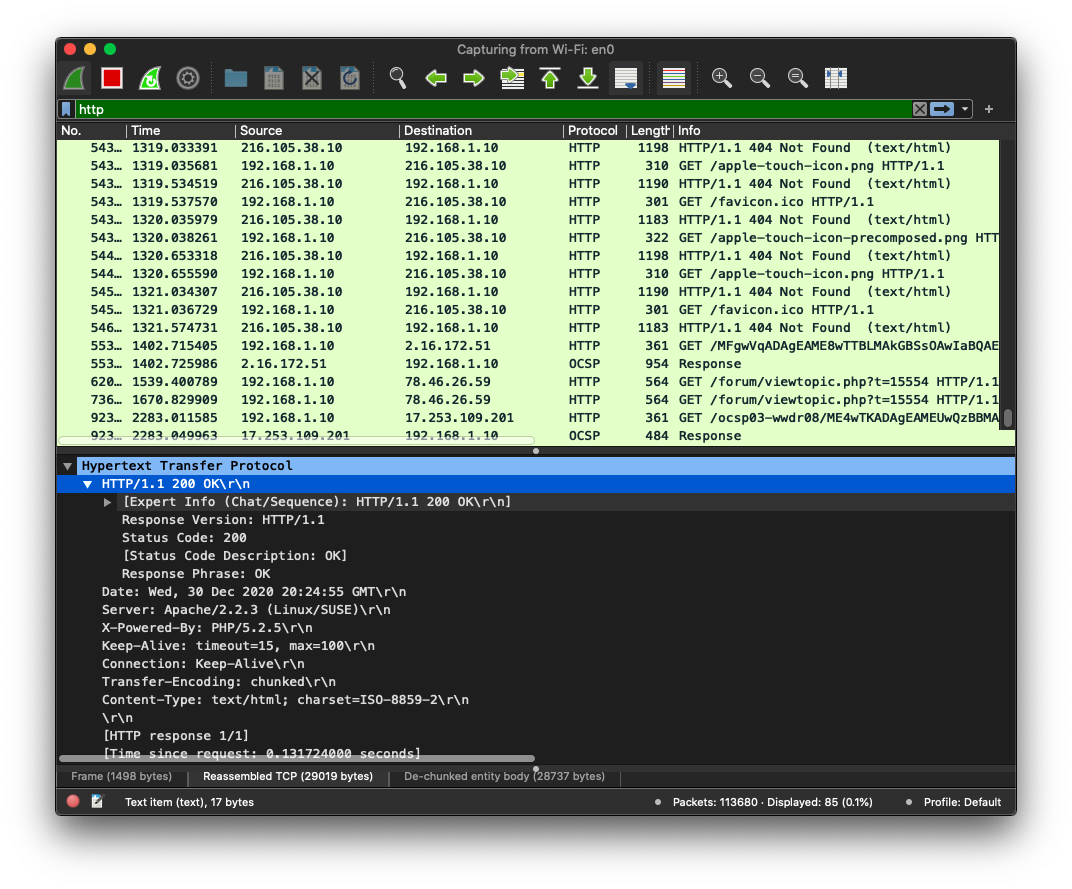
\includegraphics[width=1.0\textwidth]{img/screenshot_fis_http.png}
		\caption{Dane protokołu http}
		\label{fig:fis_http}
	\end{figure}


	\newpage
	\subsubsection{Tworzenie dekoderów}
	\indent\par
	Program Wireshark wyposażony jest w zestaw dekoderów do najczęściej wykorzystywanych protokołów. Twórcy programu
	dają jednakże możliwość tworzenia własnych. Głównym tego celem jest możliwość
	dekodowania własnych protokołów oraz reintepretacja już istniejących. Sposoby ich pisania podzielić można na 3 rodzaje.
	\begin{itemize}
		\item Opisowe -- opisana w formie tekstowej struktura pakietu oraz inne, konieczne do zdekodowania informacje.
			Wireshark posiada wbudowane wsparcie dla pisania dekoderów za pomocą notacji \texttt{ASN.1}. Wymaga to opisania
			w niej zawartości pakietu, a następnie przekompilowaniu do dekodera wraz ze szkieletem dekodera napisanym w C.
			Zazwyczaj tworzone w ten sposób dekodery wbudowane są w program Wireshark, co oznacza konieczność przekomilowywania
			całego projektu po wprowadzeniu zmian.
			Inną z dostępnych możliwości tworzenia takich dekoderów jest wykorzystanie projektu ,,WireShark Generic Dissectors'' (WSGD).
			Do instalacji programu Wireshark doinstalowywany jest plugin, który czyta napisany przez programistę opis pakietu.
		\item Skryptowe -- dekoder napisany w języku skryptowym. Wireshark posiada natywne wsparcie dla obsługi pluginów
			napisanych w języku \texttt{lua}. Język ten jest kompletny w sensie Turinga, co daje znacznie większe możliwości
			niż opisywanie struktury pakietu, wymaga jednak znajomości tego języka. Jedną z alternatyw jest tworzenie
			dekoderów w znacznie popularniejszym języku \texttt{python}, co umożliwia plugin \texttt{Pyreshark}.
		\item Kompilowane -- dekoder napisany w języku C. Jest to standardowy sposób pisania dekoderów dla programu Wireshark,
			wykorzystany przez co najmniej znaczną większość wbudowanych dekoderów. Dekodery w języku C mogą być zarówno wbudowane,
			jak i zaimplementowane jako osobne wtyczki. Do tworzenia dekoderów w języku C udostępnione zostało API \texttt{epan}.
	\end{itemize}

	Opisowe dekodery są najprostsze w implementacji, jednak działają zwykle najwolniej, a ich możliwości są ograniczone.
	Dekodery napisane w C mają największe możliwości, chociażby dlatego, że mogą korzystać z \texttt{libwireshark}. Działają zwykle
	najszybciej, a gotowy plugin łatwo jest przenieść do innej instalacji, ale ich problemem jest wyższy próg wejścia.
	Ich kod źródłowy jest zwykle najbardziej obszerny i najmniej czytelny. Kompromis pomiędzy tymi dwoma podejściami
	stanowi pisanie w języku skryptowym.



\newpage
\section{Narzędzia programistyczne}

	\subsection{Tworzenie kodu źródłowego wtyczki}
	\indent\par
	Wtyczka napisana została w języku C. Kod projektu nie wykorzystuje żadnych zewnętrzych bibliotek -- wykorzystane pliki nagłówkowe
	pochodzą ze standardowej biblioteki C oraz kodu źródłowego programu Wireshark $($\texttt{libwireshark}$)$.
	Program Wireshark używa wielu bibliotek, takich jak \texttt{qt} oraz \texttt{gthread}, ale na wyszczególnienie zasługuje biblioteka
	\texttt{glib} w wersji drugiej, której
	elementy zostały użyte w kodzie źródłowym aplikacji. \texttt{Glib2} dostarcza projektowi standardowych typów o stałym
	rozmiarze wykorzystywanych przez część używanych funkcji.

	Kod źródłowy projektu został napisany w całości w programie Vim. Jest to głównie spowodowane preferencjami autora,
	choć aby do tworzenia wtyczki wykorzystać środowisko programistyczne ze sprawdzaniem składni konieczne byłoby umieszczenie
	głównego katalogu wtyczki w projekcie Wireshark, tak aby główny plik \texttt{CMakeLists.txt} projektu znajdował się w jednym
	z nadrzędnych katalogów folderu wtyczki. Zamiast tego utworzone było dowiązanie symboliczne folderu wtyczki do katalogu
	\texttt{plugins/epan/inz}.

	Na początku prac nad wtyczką wykorzystywany był program \texttt{netcat}. Umożliwia on wysyłanie pakietów
	UDP oraz TCP na wybrany port, a także ich odbieranie.

	Podczas tworzenia wtyczki użyte zostały dwa narzędzia napisane przez autora pracy:
	\begin{itemize}
		\item \texttt{printhex} - program napisany w C służący do wyświetlania otrzymanych bajtów w zapisie szesnastkowym. Standardowo
			czyta on z \texttt{stdin} i wysyła output na \texttt{stdout}, lecz możliwe jest podanie nazwy plików wejściowego oraz wyjściowego. Narzędzie
			to wykorzystywane było podczas wczesnych prac nad wtyczką do tworzenia pakietów.
		\item \texttt{reverse} - program zamieniający kolejność bitów w masce -- przykładowo \texttt{0xFCull} na \texttt{0x3F00000000000000ull}.
			Nie posiada on żadnych dodatkowych funkcjonalności i czyta ze \texttt{stdin}. Używany był przy ustalaniu masek bitowych dla elementów pól
			,,Status'' oraz ,,Data''.
	\end{itemize}

	\subsection{Kompilacja wtyczki}
	\indent\par
	Podczas kompilacji projektu wykorzystywane jest narzędzie \texttt{cmake}. Służy ono do zarządzania procesem kompilacji,
	umożliwiając jednolity proces budowy projektu
	na każdym ze wspieranych systemów operacyjnych. Wykrywa ono konieczne do zbudowania projektu narzędzia, informując
	o brakujących, a także, tworzy skrypty kompilacyjne, które zależne są od systemu operacyjnego i konfiguracji. Na systemach Unixowych
	oznacza to zwykle generowanie plików Makefile, na systemie Windows - projektu w Visual Studio. Użycie cmake'a
	jest pierwszym krokiem standardowej kompilacji programu Wireshark oraz jego wtyczek.
	
	Do kompilacji wymagany jest kompilator do języka C. Decyzję o wykorzystaniu konkretnego narzędzia podejmuje \texttt{cmake}.
	W razie braku stosownego kompilatora \texttt{cmake} poinformuje użytkownika o problemie. Ponadto wymagany jest szereg
	bibliotek.

	Część wymagań dla Wireshark 3.4.2:
	\begin{itemize}
		\item \texttt{GLIB2} - biblioteka od GNU będąca implementacją biblioteki standardowej C wraz z wieloma rozszerzeniami.
		\item \texttt{GTHREAD2} - biblioteka do wielowątkowości od GNU.
		\item \texttt{GCRYPT} - bibliokeka kryptograficzna od GNU.
		\item \texttt{CARES} - bilbioteka do asynchronicznych zapytań DNS.
		\item \texttt{LEX} - generator analizatorów leksykalnych. Najczęściej flex.
		\item \texttt{YACC} - generatoror analizatorów składniowych. Najczęściej bison.
		\item \texttt{Perl} - interpreter oraz zestaw narzędzi do języka perl.
		\item \texttt{Python3} - interpreter oraz zestaw narzędzi do języka python w wersji 3.
		\item \texttt{M} - biblioteka do obliczeń matematycznych będąca częścią biblioteki standardowej C.
		\item \texttt{Qt5} - biblioteka do budowania przenośnych interfejsów graficznych.
	\end{itemize}

	\indent\par


\newpage
\section{Implementacja projektu}

	Dekoder został zaimplementowany jako wtyczka w języku C. Użycie języka C umożliwia analizowanie dużych zbiorów pakietów znacznie
	szybciej, niż w przypadku innych rozwiązań, a napisanie dekodera jako wtyczki ułatwia jego instalację oraz przyspiesza budowę projektu.
	Jest to zalecany przez twórców sposób implementowania dekoderów.

	Kod projektu napisany został z wykorzystaniem paradygmatu programowania funkcyjnego. Oznacza to, że kod programu bazuje na wywołaniach
	funkcji. Funkcjom przekazywane są argumenty, na których wykonują one operacje, a następnie zwracają wynik. Wywołania funkcji tworzą drzewo,
	w którym wyraźnie zaznaczona jest struktura działania programu. Jest to najbardziej naturalny sposób programowania w języku C,
	jednak pomijając ten aspekt użycie innego paradygmatu zostało uznane przez autora za zbędne i zmniejszające czytelność kodu.

	Plugin korzysta z dostarczonego przez twórców Wireshark API \texttt{epan}. Jest ono zaprojektowane pod kątem tworzenia dekoderów,
	upraszczając ich kompilację oraz umożliwiając ich poprawną rejestrację.

	TODO: opisać proces tworzenia wtyczki.

	\subsection{Wtyczka w C}
	\indent\par
	\subsubsection{Struktura programu}

	\indent\par
	Podstawę programu stanowią 3 funkcje w C, wymagane przez API \texttt{epan} do poprawnego działania dekodera. Są to:
	\begin{itemize}
		\item \texttt{int dissect()} -- funkcja zawierająca większość logiki projektu, analizująca pakiet i wyświetlająca
			pola pakietu w interfejsie graficznym programu Wireshark.
		\item \texttt{void proto\_register\_gemroc\_udp()} -- funkcja rejestrująca struktury danych pakietu GEMROC UDP.
			Wypełnianie pól tekstowych, zawierających dane i wyświetlanych przez interfejs graficzny, jest częściowo
			automatyczne. Dane zarejestrowane dzięki tej funkcji umożliwiają tą automatyzację.
		\item \texttt{void proto\_reg\_handoff\_gemroc\_udp()} -- funkcja rejestrująca dekoder. Informuje ona dekoder wyżej
			w hierarchii o zainteresowaniu określonymi pakietami. W niej znajduje się informacja, że przechwytywane pakiety
			przesyłane są protokołem UDP na porcie 48350.
	\end{itemize}

	Dwie ostatnie funkcje wywoływane są automatycznie podczas uruchamiania programu. Kod do ich wywołania generowany jest
	podczas kompilacji wtyczki przez API \texttt{epan}. Wymaga ono aby nazwy tych funkcji miały format \texttt{proto\_register\_*} oraz
	\texttt{proto\_reg\_handoff\_*}.

	\subsubsection{Funkcja \texttt{void proto\_register\_gemroc\_udp()}}

	\indent\par
	Większą część kodu funkcji \texttt{void proto\_register\_gemroc\_udp()} zajmuje definicja tablicy o nazwie \texttt{hf}.
	Jest to tablica struktur typu \texttt{hf\_register\_info}, które zawierają informacje o polach pakietu. Każdemu polu przypisana
	jest nazwa, opis, typ danych oraz nazwa służąca do filtrowania. Opcjonalnie można podać maskę, z którą dokonywany jest iloczyn logiczny
	wartości pola. Wynik jest następnie przesuwany w prawo o wartość będącą pozycją pierwszego aktywnego bitu maski.
	W tym miejscu określany jest także sposób wyświetlania danego pola. Służy do tego zestaw stałych o nazwach
	zaczynających się od \texttt{BASE\_}. Dostępne możliwości zależą od podanego wcześniej typu danych pola -- dla liczb całkowitych
	określić można przykładowo podstawę systemu liczbowego. Szczegółowe informacje na temat dostępnych stałych i ich znaczenia
	znajdują się w pliku \texttt{README.dissector} dołączonym do kodu źródłowego programu Wireshark (katalog doc projektu).
	Dwie szczególne stałe to:
	\begin{itemize}
		\item \texttt{BASE\_NONE} -- używana, gdy nie dostępny jest wybór sposobu wyświetlania.
		\item \texttt{BASE\_CUSTOM} -- informuje program Wireshark aby użył podanej przez programistę funkcji do wyświetlenia pola.
	\end{itemize}

	\begin{lstlisting}[style=CStyle]
	static hf_register_info hf[] = {
		{ &hf_packet_no,
			{ "Packet no", DISSECTOR_FILTER_NAME ".pack_no",
			  FT_UINT64, BASE_DEC, NULL, 0x0,
			  "Number of this packet", HFILL }
		},
		{ &hf_packet_status,
			{ "Status", DISSECTOR_FILTER_NAME ".status",
			  FT_UINT64, BASE_HEX, NULL, 0x0,
			  "Status containing info about asic settings", HFILL }
		},
		[...]
	};

	\end{lstlisting}

	Wireshark umożliwia napisanie własnej funkcji do wyświetlania pola. Jest to konieczne, gdy dostępne opcje okażą się niewystarczające.
	Przykładem takiej sytuacji jest konieczność dodania do pola innej wartości, czy jego przesunięcia bitowego.
	Funkcja taka przyjmuje wskaźnik na tablicę znaków, którą uzupełnia, oraz wartość pola do wyświetlenia. Tablica znaków ma długość
	\texttt{ITEM\_LABEL\_LENGTH}. W projekcie wykorzystane są dwie takie funkcje -- do pól ,,ASIC id'' oraz ,,TimeStamp ASIC''.

	Funkcja \texttt{void proto\_register\_gemroc\_udp()} rejestruje ponadto tablicę poddrzew protokołu (ang. subtree). Są one wykorzystywane
	gdy jedno pole składa się z mniejszych sekcji. Interfejs graficzny umożliwia rozwinięcie takiego pola, aby ukazać użytkownikowi jego składowe.
	Przykładem takiej sytuacji są najczęściej pola bitowe -- w projekcie pole ,,Status'' dzieli się na mniejsze podpola, takie jak
	,,Clk state'', czy ,,I2C status''. Struktura drzew określona jest w funkcji \texttt{void dissect()} --
	\texttt{void proto\_register\_gemroc\_udp()} informuje program o ich istnieniu.

	Ostatnim zadaniem funkcji jest zarejestrowanie całego protokołu. Używana do tego celu jest funkcja \texttt{proto\_register\_protocol()},
	której programista przekazuje trzy wersje nazwy protokołu: pełną, skróconą oraz nazwę do filtrowania.

	\subsubsection{Funkcja \texttt{void proto\_reg\_handoff\_gemroc\_udp()}}
	\indent\par
	Funkcja \texttt{void proto\_reg\_handoff\_gemroc\_udp()} wpisuje w tablicy dekoderów jakie dane mają być wysyłane do danego dekodera.
	Rejestracja dokonywana jest za pomocą funkcji \texttt{void dissector\_add\_uint()}. Programista podaje w niej string zawierający filter name
	danego parametru, oraz wartość, której ma on być równy. W tym projekcie jest to \texttt{"udp.port"}, który wynosić ma 48350.
	Dekoder wyższego rzędu (np. UDP) wywołuje funkcję \texttt{dissector\_try\_uint()}, bądź jej podobną, która próbuje przekazać pakiet
	kolejnemu dekoderowi. Wywoływana jest wtedy zarejestrowana za pomocą \texttt{dissector\_handle\_t create\_dissector\_handle()} funkcja
	konsumująca pakiet -- w tym projekcie \texttt{int dissect()}.

	\subsubsection{Funkcja \texttt{int dissect()}}
	\indent\par
	Główną funkcją projektu, zawierającą logikę dysekcji pakietu, jest funkcja \texttt{int dissect()}.
	\begin{lstlisting}[style=CStyleLine]
	int dissect(tvbuff_t *tvb, packet_info *pinfo, proto_tree *tree, void *data)
	\end{lstlisting}
	Konsumując pakiet buduje ona drzewo struktur danych w pakiecie i uzupełnia pola ogólnych informacji na temat pakietu. Budowanie
	drzewa dokonywane jest za pomocą zestawu funkcji udostępnionych przez API Wiresharka. Podstawę stanowi drzewo przekazane jako
	argument funkcji. Do drzewa dodawane są kolejne obiekty (ang. item), stanowiące między innymi zdefiniowane w \texttt{void proto\_register()}
	pola pakietu, choć możliwe jest także tworzenie dodatkowych pól. Przykładem takiego pola jest lista ,,Packet list''.

	Pakiet dostarczany jest funkcji jako argument typu \texttt{tvbuff\_t}. API \texttt{epan} wymaga aby wszystkie operacje
	na pakiecie dokonywane były za pomocą dostarczonych przez API funkcji. Programista nie zna więc definicji typu \texttt{tvbuff\_t}.

	Jako, że pakiet ma stałą długość, jest ona sprawdzana na początku funkcji. Jeśli jest ona różna od oczekiwanej funkcja
	kończy działanie zwracając skomsumowaną ilość danych -- 0 bajtów. Do sprawdzenia długości pakietu wykorzystywana jest funkcja
	\texttt{guint tvb\_captured\_length()}.

	Jeśli pakiet ma prawidłową długość uzupełniana jest kolumna informacji o pakiecie. Znajduje się w najwyższym oknie interfejsu
	graficznego programu Wireshark (Rys \ref{fig:col}). Służy do tego przekazywany funkcji argument
	typu \texttt{packet\_info*} oraz zestaw funkcji \texttt{col\_*}. W projekcie uzupełniane są dwa pola:
	\begin{itemize}
		\item \texttt{COL\_PROTOCOL} -- zawierające nazwę protokołu.
		\item \texttt{COL\_INFO} -- zawierające skróconą informację o pakiecie.
	\end{itemize}
	Konwencja używana przez większość dekoderów zakłada, że nazwa protokołu jest stała dla każdego pakietu, jednak skrócona
	informacja o pakiecie powinna go w jakiś sposób określać. Autor pracy uznał więc za stosowne, aby uzależnić ją
	od numeru pakietu oraz ilości danych w pakiecie.

	API programu Wireshark umożliwia czytanie danych pakietu z dowolnej jego pozycji. Służą do tego funkcje o nazwach \texttt{tvb\_get\_*}.
	Aby uzupełnić kolumnę informacji pobierane są więc z pakietu ilości danych i numeru porządkowego pakietu. Ilość danych jest także niezbędna
	w późniejszym etapie ich ekstrakcji z sekcji danych pakietu.

	\begin{figure}[h]
		\centering
			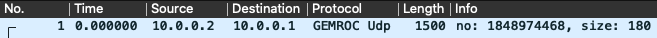
\includegraphics[width=1.0\textwidth]{img/screenshot_col.png}
		\caption{Uzupełniona kolumna protokołu}
		\label{fig:col}
	\end{figure}

	Po uzupełnieniu podstawowych informacji budowane jest drzewo pakietu. Do drzewa dodawane są kolejne pola pakietu za pomocą
	funkcji \texttt{proto\_tree\_add\_*}. Kolejność dodawania obiektów ma wpływ na kolejność wyświetlania. Rozsądnym jest więc
	dodawać pola w kolejności ich występowania w pakiecie. Dodatkowym tego atutem jest możliwość zadeklarowania zmiennej offset
	i jej zwiększania po każdym przeczytanym polu zgodnie z jego rozmarem. Inaczej konieczne byłoby podawanie pozycji pola jako
	stałej wartości przy każdym polu, a w przypadku zmiany specyfikacji protokołu przeliczanie części wartości.

	Dodanie obiektów do drzewa dokonywane jest najczęściej za pomocą funkcji \texttt{proto\_tree\_add\_item()}.
	Używa się jej dla większości typów pól, takich jak liczby całkowite, adresy, ciągi znaków, ale też dla protokołów.
	Dla pól bitowych istnieją specjalne funkcje \texttt{proto\_tree\_add\_bitmask*}. Pole bitowe tworzy automatycznie
	osobne drzewo, programista nie musi więc tworzyć go jawnie. Konieczne jest za to podanie tablicy pól składających
	się na dane pole bitowe, oraz uchwytu zapamiętującego czy dane pole jest rozwinięte, czy nie. W projekcie tablicami
	zawartości pól są \texttt{status\_fields} oraz \texttt{data\_fields}, a uchwytami zmienne poprzedzone prefiksem \texttt{ett\_}.

	W funkcji jawnie tworzone są dwa drzewa -- jedno dla całego pakietu, które jest wymagane w każdym dekoderze, oraz jedno
	dla listy danych. Umożliwia to jej zwinięcie, co biorąc pod uwagę maksymalną liczbę danych wydaje się być konieczne.
	Utworzenie nowego drzewa możliwe jest tylko na istniejącym już obiekcie. Drzewo dla całego projektu
	tworzone jest na uchwycie protokołu otrzymanym po jego rejestracji, natomiast drzewo dla listy danych tworzone jest na dodanym
	ciągu znaków podpisującym listę -- jest to napis ,,Data list''. Następnie w pętli dodawane są do niego dane pakietu jako pola bitowe $($bitmask$)$.

	Na koniec funkcja dodaje pole ilości danych ,,Data count'' i kończy działanie zwracając rozmiar pakietu, czyli ilość zużytych danych.

	\subsubsection{Pozostała część kodu}
	W projekcie, oprócz wyżej wymienionych funkcji, zaimplementowane są także dwie funkcje służące do wyświetlania pól ,,ASIC id'' oraz ,,TimeStamp ASIC''.
	Osobne funkcje do tych pól są konieczne, gdyż do pierwszego pola dodana być musi stała wartość \texttt{86}, a drugie pole zostać musi przesunięte (ang. bit shift)
	o wartość \texttt{2}. Na pozostałość kodu składają się także deklaracje:
	\begin{itemize}
		\item masek bitowych używanych przy wyciąganiu wartości niektórych pól
		\item niektórych stałych użytych w programie, takich jak nazwa bądź port, na którym przesyłany jest pakiet
		\item zmiennych pełniących funkcję uchwytów dla elementów pakietu oraz drzew
		\item tabel elementów pól bitowych
		\item makr wykorzysanych do wyświetlania informacji do debugowania
	\end{itemize}

	\subsection{Skrypty budowania oraz narzędzie \texttt{cmake}}

	Projekt kompilowany jest przy użyciu narzędzia \texttt{cmake}. Do projektu dołączony jest więc plik \texttt{CMakeLists.txt}.
	Większość jego elementów jest taka sama dla każdej wtyczki opartej o API \texttt{epan}.
	W pliku określona jest nazwa projektu, jego wersja, oraz lista plików źródłowe koniecznych do prawidłowej kompilacji wtyczki.

	Plik ten musi zostać zaimportowany przez inny plik programu \texttt{cmake}. Jest to konieczne, gdyż używa on funkcji pochodzących z kodu projektu Wireshark.
	Importowanie odbywa się przez odpowiedni wpis w pliku \texttt{CMakeListsCustom.txt}. Plik ten powinien się znajdować w głównym katalogu kodu źródłowego
	projektu Wireshark. Plik ten jest opcjonalny, dlatego może zaistnieć potrzeba jego utworzenia. Wzorem może być plik \texttt{CMakeListsCustom.txt.example}.
	W pliku \texttt{CMakeListsCustom.txt} umieścić należy względną ścieżkę do katalogu wtyczki. Wtyczka może być traktowana jako wymagana do prawidłowej kompilacji, bądź opcjonalna.
	Decyduje o tym umieszczenie jej ścieżki. Jeśli dopisana jest ona do \texttt{CUSTOM\_PLUGIN\_SRC\_DIR} brak opisanego przez nią katalogu, bądź zapisanego w nim pliku \texttt{CMakeLists.txt},
	poskutkuje błędem podczas przygotowywania skryptów kompilacyjnych. Jeśli ścieżka dopisana jest do \texttt{\_OPTIONAL\_CUSTOM\_PLUGIN\_SRC\_DIR} \texttt{cmake}
	wyświetli tylko informację o niemożności zbudowania wtyczki, natomiast dalsza kompilacja projektu, z pominięciem wskazanej wtyczki, będzie możliwa.

\newpage
\section{Testowanie projektu}

	Aplikacja testowana była na stworzonym dwóch stworzonych przez autora pakietach: \texttt{sample\_data.txt}
	i \texttt{sample\_data2.txt}, oraz dwóch zestawach pakietów, zapisanych jako pliki o rozszerzeniu pcap:
	\texttt{full.pcap} oraz \texttt{GEM\_ALU1\_ArCO2\_70\_30\_Fe55\_AM\_Th\_55\_HV\_3800\_POS\_8\_part\_015.pcap}.
	Pakiety stworzone przez autora pracy okazały się nie być zgodne ze specyfikacją, lecz umożliwiły autorowi
	wczesne eksperymenty z pisaniem dekoderów, dostarczając mu wykorzystanej później wiedzy. Pakiety były wysyłane
	i odbierane z tego samego urządzenia za pomocą narzędzia \texttt{netcat}.

	W późniejszych pracach nad projektem używane były zestawy pakietów o rozszerzeniu \texttt{.pcap}.
	Wyniki dysekcji drugiego zestawu porównywane były z danymi będącymi efektami parsowania pakietów
	przez zewnętrzne narzędzie.

	TODO: jakie narzędzie

	Dane do porównania zapisane były w pliku \texttt{GEM\_ALU1\_ArCO2\_70\_30\_Fe55\_AM\_Th\_55\_HV\_3800\_POS\_8\_part\_015.txt} oraz
	jego rozszerzonej wersji \texttt{GEM\_ALU1\_ArCO2\_70\_30\_Fe55\_AM\_Th\_55\_HV\_3800\_POS\_8\_part\_015\_more.txt}.
	z informacją o znaczeniu poszczególnych pól.

	\begin{minipage}{\linewidth}
	\begin{lstlisting}[style=CStyle,caption={Zawartość pliku *more.txt}]
	#RawDataView
	#ASIC	Channel	TimeStamp	Adc	PileUp	OverFlow	Gain	Thr	iCal	Trim	TS Asic	TS Fpga
	87	24	1948361487724	2012	0	0	249	55	50	23	13676	118918547
	87	25	1948361487756	926	0	0	249	55	50	11	13708	118918547
	87	26	1948361487700	2153	0	0	249	55	50	13	13652	118918547
	88	28	1948361504176	2189	0	0	249	55	50	11	13744	118918548
	88	29	1948361504236	1422	0	0	249	55	50	18	13804	118918548
	88	30	1948361504188	2107	0	0	249	55	50	17	13756	118918548
	88	27	1948361516912	2250	0	0	249	55	50	18	10096	118918549
	88	28	1948361516956	1556	0	0	249	55	50	11	10140	118918549
	88	29	1948361516964	965	1	0	249	55	50	18	10148	118918549
	88	30	1948361516916	2108	0	0	249	55	50	17	10100	118918549
	\end{lstlisting}
	\end{minipage}

	\begin{table}[H]
		\resizebox{\columnwidth}{!}{
		\begin{tabular}{ |c|c|c|c|c|c|c|c|c|c|c|c| }
			\hline

			ASIC & Channel & TimeStamp & Adc & PileUp & OverFlow & Gain & Thr & iCal & Trim & TS Asic & TS Fpga \\
			\hline
			87 & 24 & 1948361487724 & 2012 & 0 & 0 & 249 & 55 & 50 & 23 & 13676 & 118918547 \\
			87 & 25 & 1948361487756 & 926 & 0 & 0 & 249 & 55 & 50 & 11 & 13708 & 118918547 \\
			87 & 26 & 1948361487700 & 2153 & 0 & 0 & 249 & 55 & 50 & 13 & 13652 & 118918547 \\
			88 & 28 & 1948361504176 & 2189 & 0 & 0 & 249 & 55 & 50 & 11 & 13744 & 118918548 \\
			88 & 29 & 1948361504236 & 1422 & 0 & 0 & 249 & 55 & 50 & 18 & 13804 & 118918548 \\
			88 & 30 & 1948361504188 & 2107 & 0 & 0 & 249 & 55 & 50 & 17 & 13756 & 118918548 \\
			88 & 27 & 1948361516912 & 2250 & 0 & 0 & 249 & 55 & 50 & 18 & 10096 & 118918549 \\
			88 & 28 & 1948361516956 & 1556 & 0 & 0 & 249 & 55 & 50 & 11 & 10140 & 118918549 \\
			88 & 29 & 1948361516964 & 965 & 1 & 0 & 249 & 55 & 50 & 18 & 10148 & 118918549 \\
			88 & 30 & 1948361516916 & 2108 & 0 & 0 & 249 & 55 & 50 & 17 & 10100 & 118918549 \\

			\hline
		\end{tabular}
	}

		\caption{Pierwsze 10 rekordów pliku .txt}
		\label{tab:data}

	\end{table}

	W dalszej części procesu tworzenia wtyczki głównym zadaniem autora było zapewnienie zgodności wyników działania
	dekodera z wynikami dostarczonymi, która została finalnie zapewniona.

		\begin{figure}[H]
			\centering
				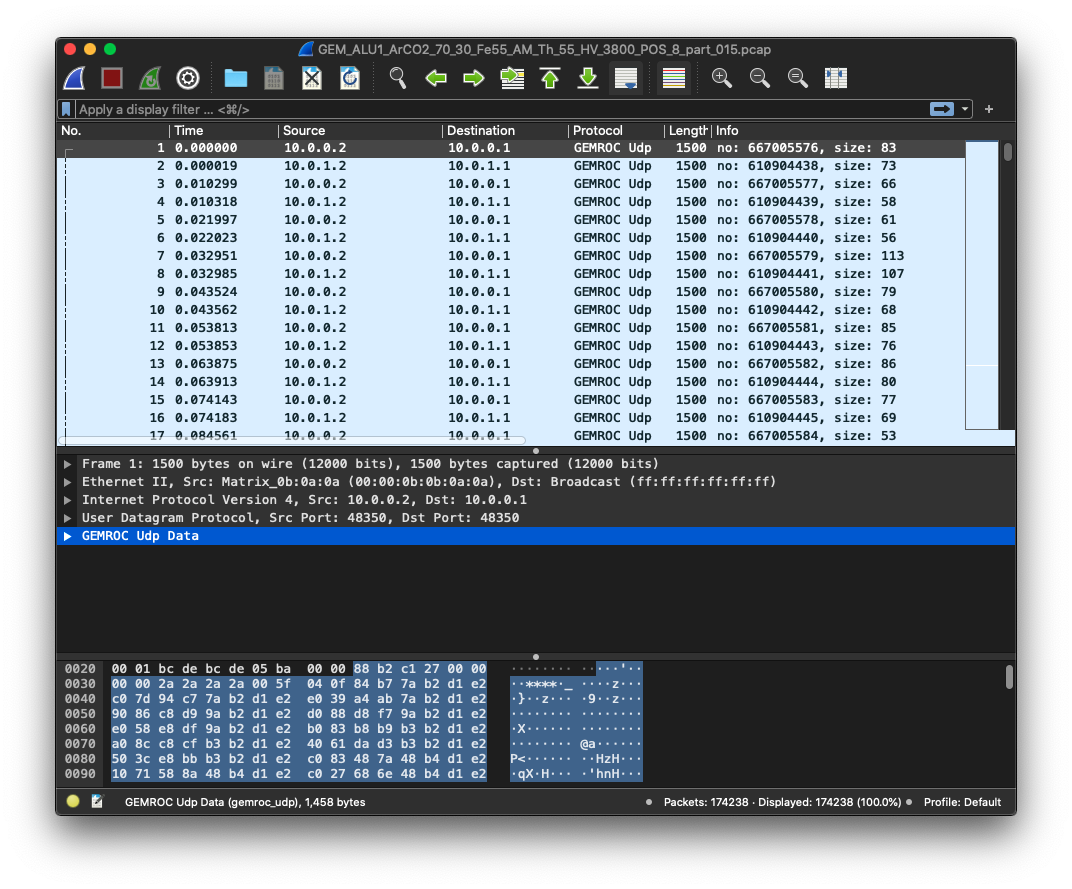
\includegraphics[width=1.0\textwidth]{img/screenshot_dissector.png}
			\caption{Ekran programu Wireshark z wgraną wtyczką}
			\label{fig:dis}
		\end{figure}

	Na pierwszym rysunku (Rys. \ref{fig:dis}) wydać wczytania do programu zawartości pliku
	\texttt{GEM\_ALU1\_ArCO2\_70\_30\_Fe55\_AM\_Th\_55\_HV\_3800\_POS\_8\_part\_015.txt}.
	W górnej części interfejsu graficznego zauważyć można, że pakiety są poprawnie rozpoznawane i przesyłane do właściwego dekodera, gdyż
	kolumny ,,Protocol'' oraz ,,Info'' wypełnione są poprawnie. Plik zawiera dwie zazębiające się transmisje, dlatego co drugi pakiet ma kolejny numer.
	Na najniższej pozycji w stosie dekoderów znajduje się protokół ,,GEMROC Udp''.

	Poniżej widać efekt wczytania tego samego pliku do instalacji programu Wireshark niezawierającej wtyczki (Rys. \ref{fig:no_dis}).
	Zamiast dekodera GEMROC Udp ostatnim poziomem są surowe dane protokołu Udp. Można je przeczytać z najniższego okna programu,
	lecz uzyskanie z niego informacji wymaga ręcznego przeliczania wartości pól.

		\begin{figure}[H]
			\centering
				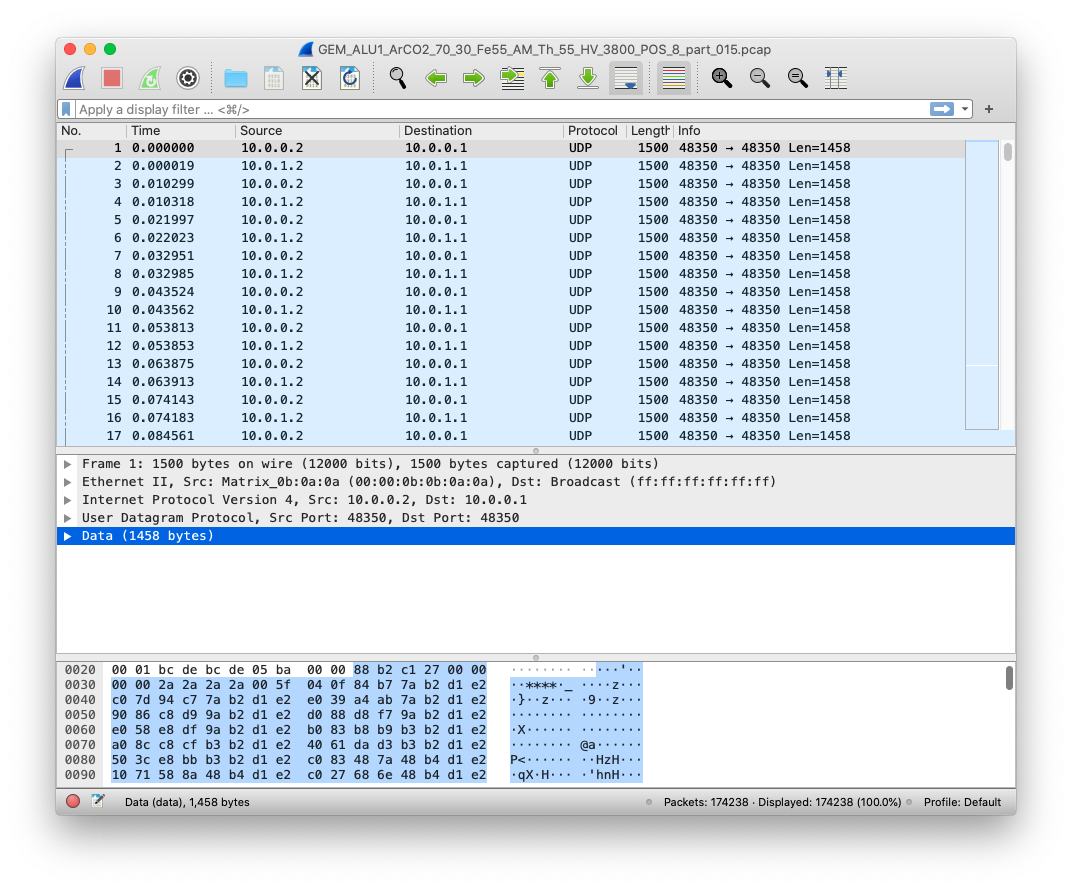
\includegraphics[width=1.0\textwidth]{img/screenshot_no_dissector.png}
			\caption{Ekran programu Wireshark bez wtyczki}
			\label{fig:no_dis}
		\end{figure}


	Po rozwinięciu protokołu ,,GEMROC Udp'' użytkownikowi ukazuje się zawartość pakietu, na którą
	składają się 4 pola: ,,Packet no'', ,,Status'', ,,Data list'' oraz ,,Data count''.
	Zawartość tą widać na kolejnym rysunku (Rys. \ref{fig:dis_pack}).

		\begin{figure}[H]
			\centering
				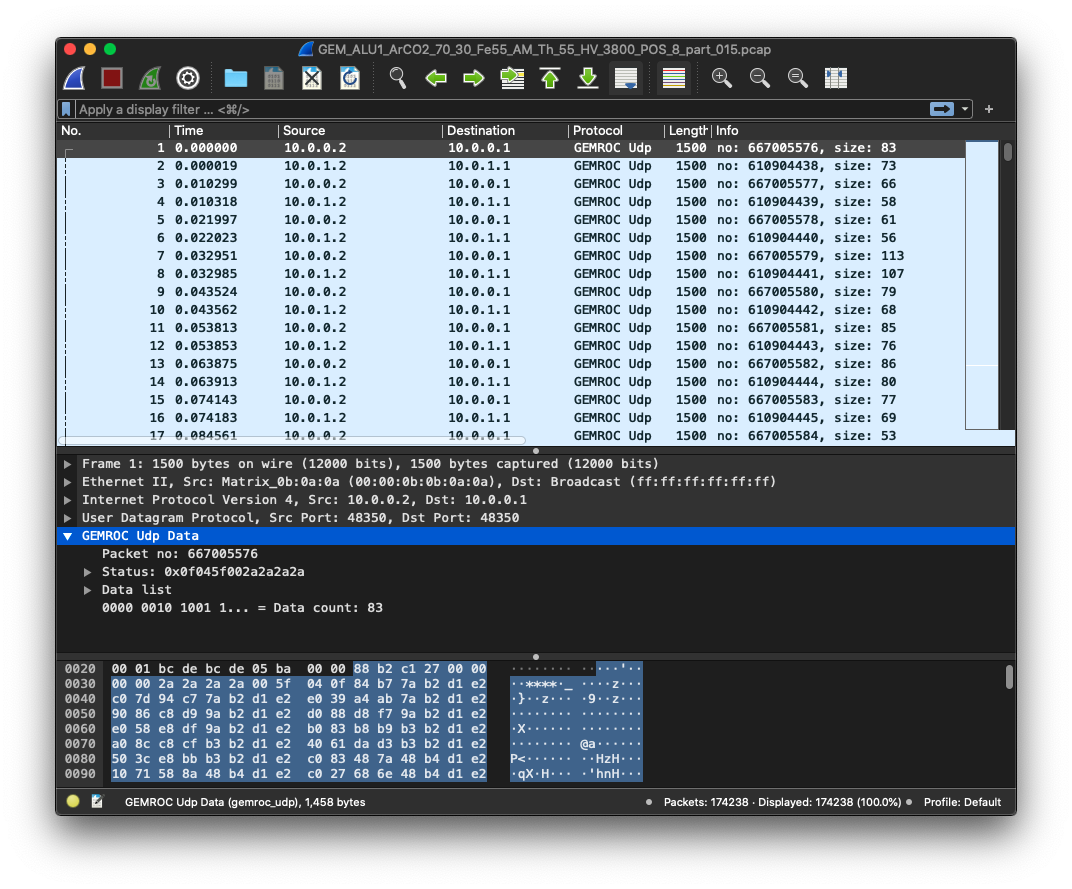
\includegraphics[width=1.0\textwidth]{img/screenshot_dissector_list.png}
			\caption{Zawartość pierwszego pakietu}
			\label{fig:dis_pack}
		\end{figure}

	Pierwsze z pól -- ,,Packet no'' -- zawiera wartość zgodną z podaną w skróconym opisie pakietu, zawartym w kolumnie ,,Info''. Kolejne pole -- ,,Status'' --
	wyświetla odpowiedni 64-bitowy fragment pakietu w notacji szesnastkowej. Aby poznać szczegółową zawartość konieczne jest jego rozwinięcie (Rys. \ref{fig:dis_status}).

		\begin{figure}[H]
			\centering
				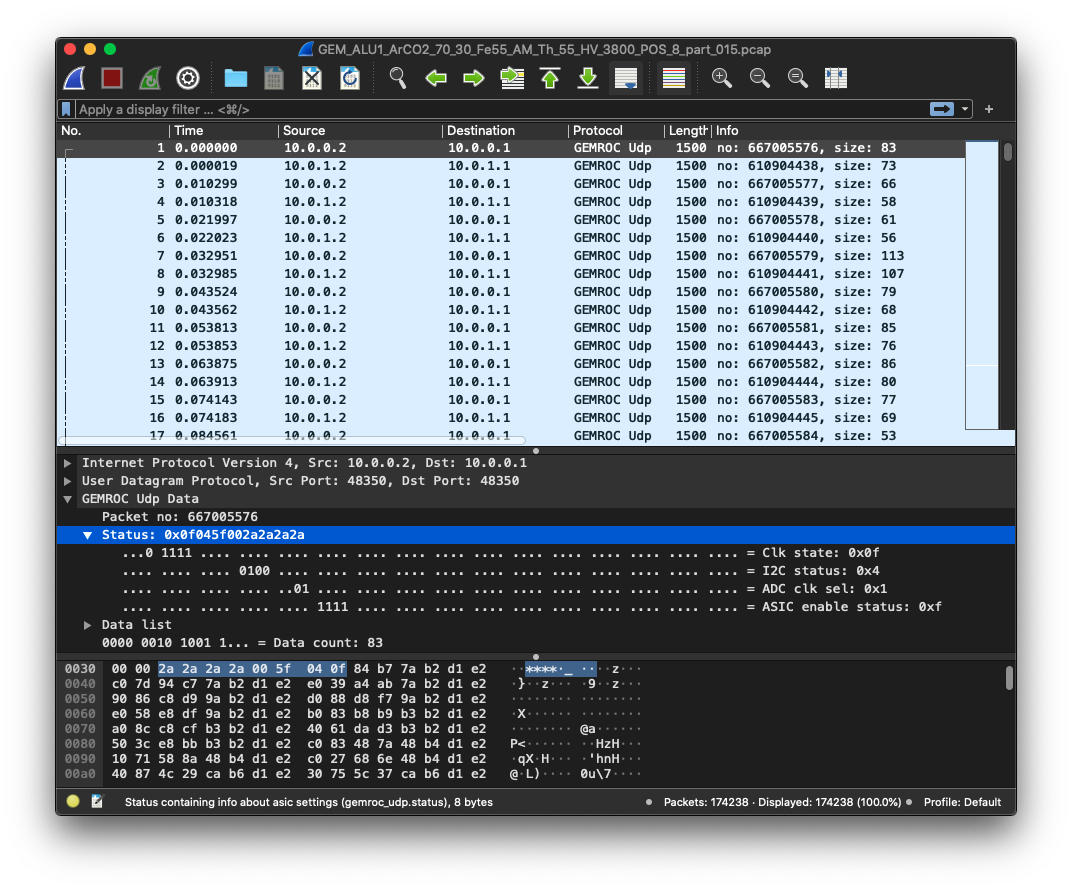
\includegraphics[width=1.0\textwidth]{img/screenshot_dissector_status.png}
			\caption{Zawartość pola ,,Status''}
			\label{fig:dis_status}
		\end{figure}

	Pole ,,Status'' zawiera cztery elementy: ,,Clk state'', ,,I2C status'', ,,ADC clk sel'' oraz ,,ASIC enable status''. Dla każdego elementu
	pola zaznaczone są wchodzące w jego skład bity. Jest to domyślny sposób wyświetlania wartości pola gdy jest ono uzyskiwane z użyciem maski.

	Kolejnym elementem pakietu jest rozwijana lista danych ,,Data list'' o długości zależnej od zawartości pakietu. Jej rozwinięcie ukazuje użytkownikowi
	listę ponumerowanych danych (Rys. \ref{fig:dis_data_list}).

		\begin{figure}[H]
			\centering
				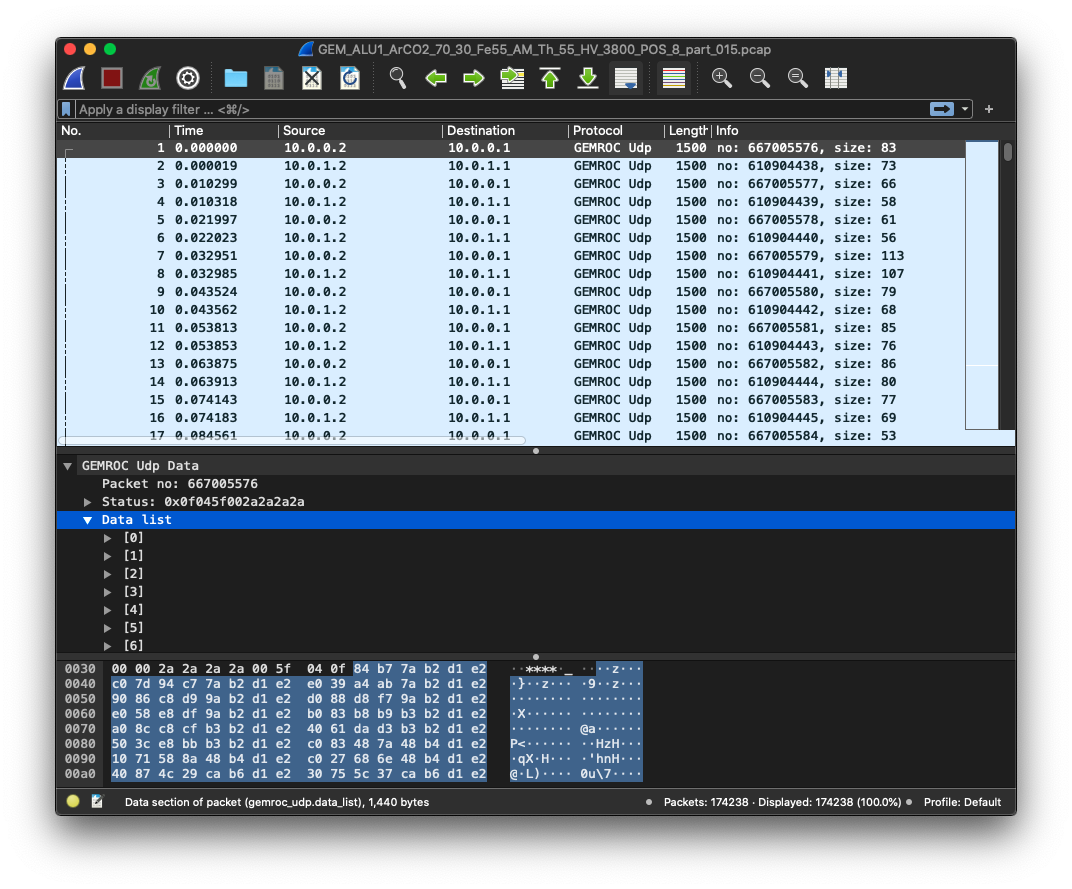
\includegraphics[width=1.0\textwidth]{img/screenshot_dissector_data_list.png}
			\caption{Lista danych pakietu}
			\label{fig:dis_data_list}
		\end{figure}

	Dane listy, podobnie jak pole status, są polem bitowym. Każdy element wymaga więc osobnego rozwinięcia. Biorąc pod uwagę średnią długość
	listy ułatwia to poruszanie się po niej. Każdy element składa się z pól ,,ADC'', ,,TimeStamp FPGA'', ,,TimeStamp ASIC'', ,,Channel id'', ,,ASIC id'',
	,,PileUp'' oraz ,,OverFlow''.

		\begin{figure}[H]
			\centering
				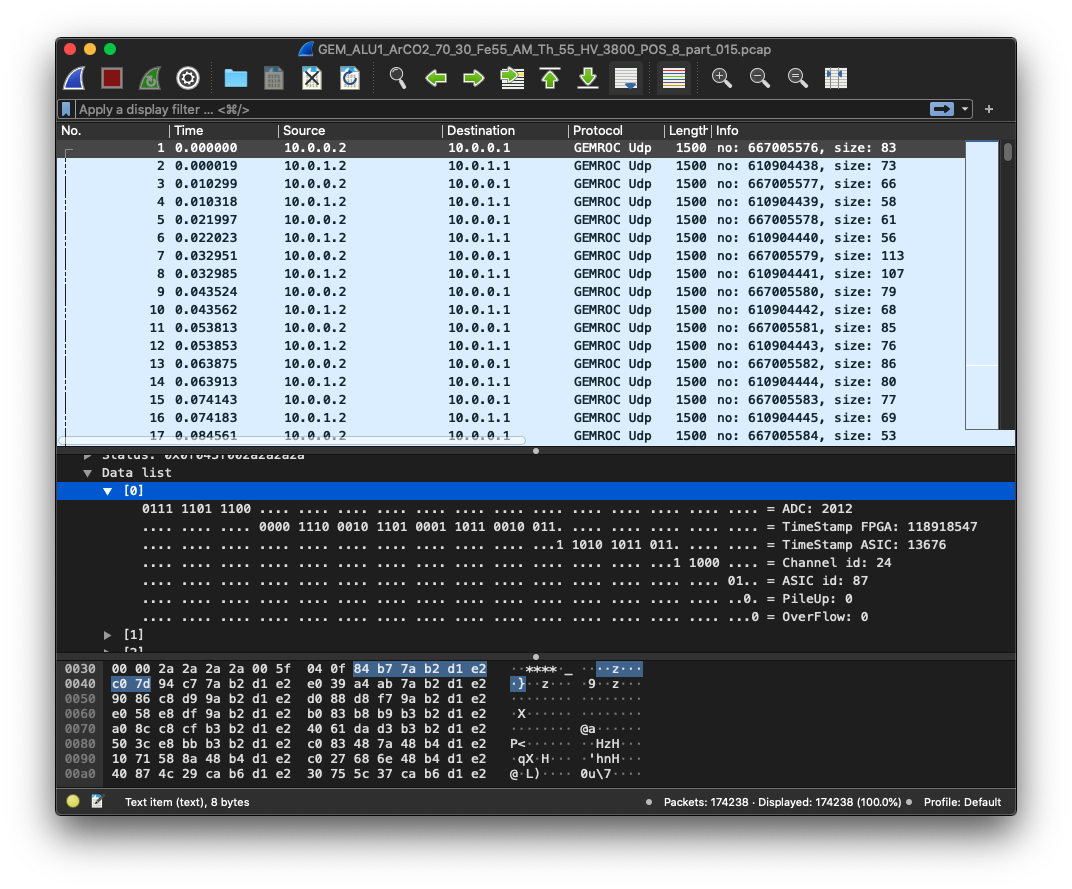
\includegraphics[width=1.0\textwidth]{img/screenshot_dissector_data.png}
			\caption{Dane pakietu}
			\label{fig:dis_data}
		\end{figure}

	Dane uzyskane z programu (Rys. \ref{fig:dis_data}) zgodne są z oczekiwanymi wartościami (Tab. \ref{tab:data}).

	Ostanim polem pakietu jest ,,Data count''. Zapisane jest one na 13 bitach, użyta została więc maska na liczbie 16-bitowej.
	Wartość ta także zgodna jest z oczekiwaniami.

	Projekt testowany był również na zestawie danych \texttt{full.pcap}.

	TODO: coś o czasie działania.

	\subsection{Wirtualny kontener -- \texttt{Docker}}

	Do projektu dołączony jest plik Dockerfile umożliwiający uruchomienie programu Wireshark wraz z zainstalowaną wtyczką
	na wirtualnym kontenerze. Kontener oparty jest o system \texttt{Debian 10} i instaluje Wireshark w wersji 3.4.2

	Po uruchomieniu kontener działa jako serwer, z którym połączyć się można za pomocą komendy \texttt{ssh}.
	Obsługuje on \texttt{X11 Forwarding}, dzięki czemu możliwe jest korzystanie z aplikacji w trybie graficznym.
	Poza plikiem \texttt{Dockerfile} stworzony został skrypt budujący i uruchamiający kontener, a także plik
	\texttt{README.md} zawierający instrukcje jak korzystać ze skryptu.

	Na kontenerze testowana była kompatybilność wtyczki z różnymi wersjami Wireshark, a także jej przenośność pomiędzy
	różnymi systemami operacyjnymi.

	Wtyczka kompiluje się poprawnie przy użyciu kodu źródłowego Wireshark w wersji 3.4.0 lub nowszej (ostatnia testowana
	wersja oznaczona jest jako \texttt{v3.5.0rc0-451-ga9ce232c3769}). W przypadku starszych wersji kodu Wireshark
	(testowane z użyciem wersji 2.6.10) kompilacja kończy się z kilkoma ostrzerzeniami o niekomplatybilnych typach przy
	wywołaniu kilku funkcji, lecz niekompatybilność dotyczy tylko kwalifikatora (ang. qualifier) \texttt{const}
	i nie uniemożliwia korzystania z projektu.

	Wtyczka przenośna jest tylko pomiędzy wersjami programu Wireshark o różnej ostatniej liczbie numeru wersji.
	Przykładowo dekoder zbudowany przy użyciu kodu źródłowego w wersji 3.4.0 współpracuje poprawnie ze wszystkimi wersjami
	3.4.

	Niemożliwe jest przenoszenie wtyczki pomiędzy systemami operacyjnymi o braku kompatybilności plików obiektowych.
	Oznacza to, że wtyczka kompilowana na systemie operacyjnym Linux nie będzie działać na systemie Windows.
	Kompatybilność taka zapewniona być może w przypadku systemów o wspólnym jądrze. Dekoder testowany był
	pomiędzy systemami \texttt{Ubuntu} oraz \texttt{Debian}. Projekt skompilowany na jednym systemie działał poprawnie
	na drugim i odwrotnie.

\newpage
\section{Tworzenie własnych dekoderów z wykorzystaniem szablonu}

	Do projektu dołączony jest także szablon wtyczki-dekodera wraz z instrukcją na temat tworzenia własnych dekoderów.
	W skład repozytorium szablonu wchodzą następujące pliki:
	\begin{itemize}
		\item \texttt{packet-template.c} - plik zawierający szablon działającego dekodera.
		\item \texttt{packet-template-bare.c} - plik zawierający okrojony szablon, niemożliwy do przekompilowania.
		\item \texttt{CMakeLists.txt} - plik programu \texttt{cmake} służący do kompilacji projektu.
		\item \texttt{README.md} - plik zawierający instrukcję tworzenia, kompilacji, testowania oraz instalacji dekoderów.
	\end{itemize}

	Instrukcja napisana w formacie \texttt{Markdown} zawiera krótki poradnik tworzenia dekodera. Bazuje ona na informacjach
	zdobytych przez autora podczas implementowania dekodera pakietów \texttt{GEMROC UDP}. W sposób znacznie krótszy,
	niż przeznaczony do tego dokument \texttt{README.dissector}, omawia ona strukturę oraz działania dekodera pakietów
	do programu Wireshark i zaimplementowanego w języku C. Dokument \texttt{README.dissector} jest jednak konieczny podczas
	tworzenia dekodera -- w instrukcji nie zostało opisanych wiele funkcji API \texttt{epan}, jedynie część z nich jest
	wspomnianych.

	Pliki \texttt{packet-template.c} oraz \texttt{packet-template-bare.c} napisane są z myślą o wykorzystaniu ich w trakcie
	pisania nowego dekodera pakietów. \texttt{packet-template.c} zawiera projekt prostego dekodera do pakietów składających
	się z dwóch segmentów: \texttt{id} oraz \texttt{data}. Segment \texttt{data} jest dodatkowo podzielny na dwie mniejsze
	części:
	\begin{itemize}
		\item bity od 20 do 31 to pole \texttt{data1}
		\item bity od 0 do 19 to pole \texttt{data2}
	\end{itemize}

	Dodatkowo wartość pola \texttt{data2} powinna zostać zwiększona o 2 przy wyświetlaniu. Taka specyfikacja protokołu
	miała na celu pokazać jak najwięcej opcji podczas tworzenia dekodera, będąc jednocześnie nieskomplikowaną.
	Umożliwia to chociażby pokazanie zasady działania masek bitowych, czy własnych funkcji wyświetlających pola protokołu.

	Plik \texttt{packet-template-bare.c} zawiera okrojoną wersję kodu źródłowego dekodera, której nie można przekompilować
	do działającej wtyczki. Plik ten miał być w zamyśle autora punktem startowym do pisania własnego dekodera, a także
	pokazywać część wspólną kodu postawowych dekoderów, ułatwiając zrozumienie początkującemu programiście.

	Plik \texttt{CMakeLists.txt}, poza umożliwianiem przekompilowania dekodera zapisanego w pliku \texttt{packet-template.c},
	użyty zostać może w projekcie nowego dekodera. Szczegóły adaptowania tego pliku w nowym projekcie zamieszczone są w instrukcji.



\newpage
\section{Dodatek}

	TODO: napisać dodatek (dodatkowe programy i ogólnie wszystko co dodatkowe)

\newpage
\section{Podsumowanie}

	TODO: podsumowanie.

\newpage
\bibliographystyle{srt}
\begin{thebibliography}{99}

	\bibitem{WGDS}
		http://wsgd.free.fr [dostęp: 30.12.2020]

	\bibitem{Packet analyzer}
		https://en.wikipedia.org/wiki/Packet\_analyzer [dostęp: 02.01.2021]

	\bibitem{WSGD tutorial}
		https://wintermade.it/blog/posts/how-to-write-generic-dissectors-in-wireshark.html

	\bibitem{Lua dissectors}
		https://wiki.wireshark.org/Lua/Dissectors

	\bibitem{Python dissectors}
		https://wiki.wireshark.org/Python

	\bibitem{ASN.1 dissectors}
		https://www.wireshark.org/docs/wsdg\_html\_chunked/Asn1DissectorRequirements.html


\end{thebibliography}


\vspace{85mm}


\end{document}


